\chapter{Verification of Composite Field Arithmetic Circuits} \label{ch:cf}

As an effort to reduce the high implementation costs, 
a methodology that designs arithmetic circuits over composite field is proposed \cite{phdpaar:1994},
where the finite field $\mathbb{F}_{2^k}$ is decomposed as $\mathbb{F}_{(2^m)^n}$, for a $k = m\cdot n$, 
and the arithmetic operations are then performed over $\mathbb{F}_{(2^m)^n}$. 
The decomposition introduces a hierarchy (modularity) in the design by lifting the ground field from $\mathbb{F}_2$
(bits) to $\mathbb{F}_{2^m}$ (words). This results in impressive area and delay
savings over large finite fields \cite{phdpaar:1994} \cite{cfmulti:1996} \cite{cf:2003}.  

The hierarchy of composite field circuits also introduces a challenge to verify such problems: 
both word-level and bit-level information are contained in the designs, which are not able to 
be solved by any contemporary technique.

This chapter addresses the implementation verification of such arithmetic circuits. 
We formulate the verification problem as an (radical) ideal membership test at different abstraction levels
and then apply approaches presented in Chapter \ref{ch:date} to solve it, i.e., conducting a polynomial reduction.

Our approach is based on the known field decomposition information and the
circuit hierarchy. 
%The composite field decomposition is actually derived from the original
%specification, and the multiplier is then custom designed while preserving the hierarchy. 
We utilize this information to: 
\begin{itemize}
	\item first verify the correctness of lower-level building-blocks (adders and
			multipliers) over the ground field $\mathbb{F}_{2^m}$; 
	\item then verify the overall function at the higher-level over the extension field $\mathbb{F}_{(2^m)^n}$. 		
\end{itemize}

Using our approach, we are able to prove the correctness of finite field circuits for up to $1024$-bit 
with decomposition $\mathbb{F}_{(2^{32})^{32}}$.

%%%%%%%%%%%%%%%%%%%%%%%%%%%%%%%%%%%%%%%%%%%%%%%%%%%%%%%%%
%%%%%%%%%%%%%%%%%%%%%%%%%%%%%%%%%%%%%%%%%%%%%%%%%%%%%%%%%
%%%%%%%%%%%%%%%%%%%%%%%%%%%%%%%%%%%%%%%%%%%%%%%%%%%%%%%%%
\section{Circuit Designs over Composite Fields}
The finite field $\mathbb{F}_{2^k}$ is a $k$-dimensional vector space over the
sub-field $\mathbb{F}_2$. If $k = m\cdot n$, the field $\mathbb{F}_{2^k}$
can be decomposed as $\mathbb{F}_{(2^m)^n}$. Such a field representation is
called a {\bf composite field}, and it is constructed as a $n$-dimensional 
extension of the sub-field $\mathbb{F}_{2^m}$. The subfield $\mathbb{F}_{2^m}$ is
called the ground field. Note that we have $\mathbb{F}_2 \subset \mathbb{F}_{2^m}
\subset \mathbb{F}_{(2^m)^n}$.  

According to Theorem \ref{the:unique}, there exists an unique field of size $p^{k}$. 
This implies that $\mathbb{F}_{2^k}$ is isomorphic to
$\mathbb{F}_{(2^m)^n}$ when $k = m\cdot n$,  and due to this isomorphism,
it is possible to derive one field representation from the other. 
The principle of constructing a composite field is described in \cite{phdpaar:1994}. 
Here we derive concrete steps for circuit design purpose.


\begin{Definition}
A {\bf primitive polynomial} $P(x)$ is a polynomial with coefficients in $\mathbb{F}_2$ which has a root $\alpha$ $\in$ $\mathbb{F}_{2^k}$
such that \{$0$, $1$, $\alpha$, $\alpha^2$, $\cdots$, $\alpha^{2^k-2}$\} is the set of all elements in $\mathbb{F}_{2^k}$, 
where $\alpha$ is a {\bf primitive element} of $\mathbb{F}_{2^k}$. 
\end{Definition}

The only difference between primitive polynomials and irreducible polynomials is whether they can generate all distinct elements 
of a finite field $\mathbb{F}_{2^k}$.
Primitive polynomials can generate all elements with a primitive element of $\mathbb{F}_{2^k}$ while irreducible polynomials 
cannot generate all elements of $\mathbb{F}_{2^k}$.

Recall that to construct a finite field $\mathbb{F}_{2^k}$, we need a primitive
polynomial $P(x) \in \mathbb{F}_2[x]$ of degree $k$. Similarly, to construct
$\mathbb{F}_{(2^m)^n}$, we require a primitive polynomial, of degree $n$, with
coefficients from the ground field $\mathbb{F}_{2^m}$. Given $\mathbb{F}_{2^k}$ and
$P(x)$, the primitive polynomial of the composite field can be easily
derived. We will use the following notation:

\begin{itemize}
\item  Let $P(x)$ denote the given primitive polynomial of general
  field  $\mathbb{F}_{2^k}$, and $\alpha$ be the primitive root, i.e. $P(\alpha)=0$.  
\item Let $Q(x)$ denote the primitive polynomial of ground field
  $\mathbb{F}_{2^m}$, and $\beta$ be the primitive root of $\mathbb{F}_{2^m}$,
  i.e. $Q(\beta)=0$. Note that $Q(x)$ is a degree $m$ primitive
  polynomial over $\mathbb{F}_{2}$ so it is also known. 
\item Let $R(x)$ denote the primitive polynomial of composite field
  $\mathbb{F}_{(2^m)^n}$, and $\gamma$ be the primitive root,
  i.e. $R(\gamma)=0$. This polynomial $R(x)$ has to be derived. 
\end{itemize}

%To construct $R(x)$, we hae the following result 
\begin{Lemma}
From \cite{cf:2003}: Let $\mathbb{F}_{2^k}$ be decomposed as $\mathbb{F}_{(2^m)^n}$
where $k = m\cdot n$. Let $\gamma$ be the primitive root of the field $\mathbb{F}_{(2^m)^n}$. 
Then 
\begin{equation}
R(x)=\prod_{i=0}^{i=n-1}(x_i+\gamma^{2^{m \cdot i}})
\end{equation}
\end{Lemma}

Since $\mathbb{F}_{2^k}$ is isomorphic to $\mathbb{F}_{(2^m)^n}$, $\alpha$ and
$\gamma$ are actually the same elements. 
%Therefore $P(x)$ and $R(x)$
%are minimal polynomials of the same element, but w.r.t. different ground fields, $GF(2)$ and
%$GF(2^m)$ respectively \cite{cf:2003}.  
Now let us consider the representation of an element $A$ in $\mathbb{F}_{2^k}$ and its corresponding
representation in the composite field. 

\begin{itemize}
\item Any element $A \in \mathbb{F}_{2^k}$ is represented as:
\begin{equation}
A=\sum_{i=0}^{i=k-1}a_i \cdot \alpha^i, a_i \in \mathbb{F}_{2}, \text{and}\	 P(\alpha) = 0
\end{equation}
\item The same element $A \in \mathbb{F}_{(2^m)^n}$ is represented as:
\begin{equation}
A=\sum_{i=0}^{i=n-1}A_i \cdot \gamma^i, A_i \in \mathbb{F}_{2^m}, \text{and} \	 R(\gamma) = 0
\end{equation}

\item
Now we have to represent the element $A_i$ from above in the ground
field $\mathbb{F}_{2^m}$:
\begin{equation}
A_i=\sum_{j=0}^{j=m-1}a_{ij} \cdot \beta^j, a_{ij} \in \mathbb{F}_{2}, \text{and} \	 Q(\beta) = 0
\end{equation}

\end{itemize}

Now we need to find the relationship between the primitive roots
$\alpha$ and $\beta$ (or between $\gamma$ and $\beta$, since $\alpha =\gamma$), 
so as to be able to map the elements from $\mathbb{F}_{2^k}$ to $\mathbb{F}_{(2^m)^n}$. 
We have the following result \cite{cf:2003}:

\begin{Theorem}\label{thm:gamma}
For $\gamma \in \mathbb{F}_{(2^m)^n}$, and $\beta=\gamma^{\omega}$, where $\omega=(2
^{m \cdot n}-1)/(2^m-1)$, then we have $\beta \in \mathbb{F}_{2^m}$. In other
words: 
\begin{equation}
\beta=\alpha^{(2^{m \cdot n}-1)/(2^m-1)}=\gamma^{(2^{m \cdot n}-1)/(2^m-1)} \label{eqn:relation}
\end{equation}

\end{Theorem}

The above result states the following: Since $\gamma$ is a primitive
root, it can be used to generate all the non-zero elements of $\mathbb{F}_{(2^m)^n}$. 
Moreover, $\beta$ is a primitive root of the ground field $\mathbb{F}_{2^m}$, 
which is a sub-field of $\mathbb{F}_{(2^m)^n}$ ( i.e. $\mathbb{F}_{2^m}
\subset \mathbb{F}_{(2^m)^n}$); so $\beta \in \mathbb{F}_{(2^m)^n}$. Therefore
an exponent of $\gamma$ can be used to generate $\beta$ as
$\beta=\gamma^{\omega}$, where $\omega$ is given in Theorem
\ref{thm:gamma}. Now we know all the relationships between $\alpha,
\beta, \gamma$, and we are ready to perform the decomposition. 

\begin{Example}
As an example, let us reconsider the field $\mathbb{F}_{2^4}$ and decompose it
as $\mathbb{F}_{(2^2)^2}$. Let $P(x) = x^4 + x^3 + 1$ and $P(\alpha)=0$. We
need to perform the following steps:

\begin{enumerate}
\item 
Derivation of $R(x)$:
\begin{eqnarray}
R(x)&=&\prod_{i=0}^{i=1}(x+\gamma^{2^{2 \cdot i}}) \nonumber \\
&=&(x+\gamma)\cdot (x+\gamma^{2^2})               \nonumber \\
&=&x^2+(\gamma^4+\gamma) \cdot x+\gamma^5          
\end{eqnarray}
Notice that $R(\gamma) = \gamma^2 + (\gamma^4+\gamma) \cdot \gamma+\gamma^5 =0$.
\item 
Representation of element $A \in \mathbb{F}_{(2^2)^2}$:
\begin{eqnarray}
A& = & \sum_{i=0}^{i=1}A_i \cdot \gamma^i, A_i \in \mathbb{F}_{2^2}\nonumber \\
 & = & A_0 +A_1 \cdot \gamma
\end{eqnarray}
\item 
Representation of $A_0, A_1$ in $\mathbb{F}_{2^m}$:
\begin{eqnarray}
A_0=a_{00}+a_{01} \cdot \beta \nonumber \\
A_1=a_{10}+a_{11} \cdot \beta
\end{eqnarray}
where $a_{ij}\in \mathbb{F}_2$. $Q(x)$ can be any degree $m=2$ primitive
polynomial in the ground field  $\mathbb{F}_{2^2}$. Let us take $Q(x)=x^2+x+1$. 

\item Now we can substitute $A_0, A_1$ into $A$ as follows:
\begin{eqnarray}
A&=&\sum_{i=0}^{i=1}(\sum_{j=0}^{j=1}a_{ij} \cdot \beta^j) \cdot \gamma^i \nonumber \\
&=&a_{00}+a_{01}\cdot \beta+(a_{10}+a_{11}\cdot \beta)\cdot \gamma   \end{eqnarray}
where each $a_{ij} \in \mathbb{F}_2$. From Eqn. (\ref{eqn:relation}), we
have: $\beta=\alpha^5=\gamma^5$. We then substitute $\beta$ and
$\gamma$ with $\alpha$ to obtain:
\begin{eqnarray}
A&=&\sum_{i=0}^{i=1}(\sum_{j=0}^{j=1}a_{ij} \cdot \beta^j) \cdot \gamma^i \nonumber \\
&=&a_{00}+a_{01}\cdot \alpha^5+(a_{10}+a_{11}\cdot \alpha^5)\cdot \alpha \nonumber 
\end{eqnarray} 
Since $P(x)=x^4+x^3+1$ with $P(\alpha)=0$, we have
\begin{equation}\label{a}
A \pmod {P(\alpha)}=a_{00}+a_{01}+a_{11}+(a_{01}+a_{10}+a_{11})\cdot \alpha+a_{1
1} \cdot \alpha^2+(a_{01}+a_{11})\cdot \alpha^3   
\end{equation}

\item The same element $A \in \mathbb{F}_{2^4}$ is represented as:
\begin{equation}\label{aa}
A=a_0+a_1\cdot \alpha+a_2\cdot \alpha^2+a_3\cdot \alpha^3 
\end{equation}

\item Since Eqns. \ref{a} and \ref{aa} represent the same element, we
  can match the coefficients of the the polynomials to obtain:
\begin{eqnarray}
a_0&=&a_{00}+a_{01}+a_{11} \nonumber \\
a_1&=&a_{01}+a_{10}+a_{11} \nonumber \\
a_2&=&a_{11} \nonumber \\
a_3&=&a_{01}+a_{11} \nonumber
\end{eqnarray}

This mapping can also be reversed and represented as a matrix $T$:
\begin{center}
$\begin{bmatrix} a_{00}\\ a_{01} \\a_{10} \\ a_{11}\end{bmatrix}
=
\begin{bmatrix} 1 & 0 & 0 & 1\\ 0 & 0 & 1 & 1\\ 0 & 1 & 0 & 1\\ 0 & 0
  & 1 & 0 \end{bmatrix} 
\begin{bmatrix} a_0\\ a_1 \\a_2 \\ a_3\end{bmatrix}$
\end{center}
\end{enumerate}

Now we have successfully derived the composite field representation
$\mathbb{F}_{(2^2)^2}$ from $\mathbb{F}_{2^4}$. The element $A \in \mathbb{F}_{2^4}$ is
represented as $A = a_0 + a_1 \alpha + a_2 \alpha^2 + a_3 \alpha^3$,
where $P(\alpha) = 0$. The same element $A$ is represented in $\mathbb{F}_{(2^2)^2}$ as:
\begin{eqnarray}
A&=&A_0+A_1 \cdot \alpha \nonumber \\
A_0&=&a_{00}+a_{01} \cdot \alpha^5 \nonumber \\
A_1&=&a_{10}+a_{11} \cdot \alpha^5 \nonumber \\
a_{00}&=&a_0+a_3 \nonumber \\
a_{01}&=&a_2+a_3 \nonumber \\
a_{10}&=&a_1+a_3 \nonumber \\
a_{11}&=&a_2 \nonumber 
\end{eqnarray}

In the above equations, $\alpha = \gamma$ and $R(\gamma) = 0$. 
\end{Example}

Multiplication $A\cdot B \pmod{ P(x)}$ over $\mathbb{F}_{2^4}$ can now be
performed over the decomposition $\mathbb{F}_{(2^2)^2}$, where $A = A_0 +
A_1\gamma, B = B_0 + B_1 \gamma$ and  the modulus is taken over
$R(\gamma)$. Such a design is shown in Figure \ref{fig:mas22}, where 
$a_0, a_1,a_2,a_3, b_0,b_1,b_2,b_3$ are primary inputs. After
a suitable transformation, {\it composite field} inputs are obtained as
$a_{00},a_{01},a_{10},a_{11},b_{00},b_{01},b_{10},b_{11}$. $A_0,A_1,B_0,B_1$
are $2$-bit buses. Correspondingly, each block in Fig.\ref{fig:mas22}
internally represents a $2$-bit operation: $\times$ represents $2$-bit
{\it multiplication}  and $+$ represents $2$-bit {\it addition} over
the ground field. 
%Our objective is to verify the correctness of
%such composite field multipliers. 
A logic circuit for a $4$-bit {\it Mastrovito} multiplier over {\it finite field} $\mathbb{F}_{2^4}$ is illustrated in Fig.\ref{fig:mas4}.

\begin{figure}[htb]
	\begin{center}
	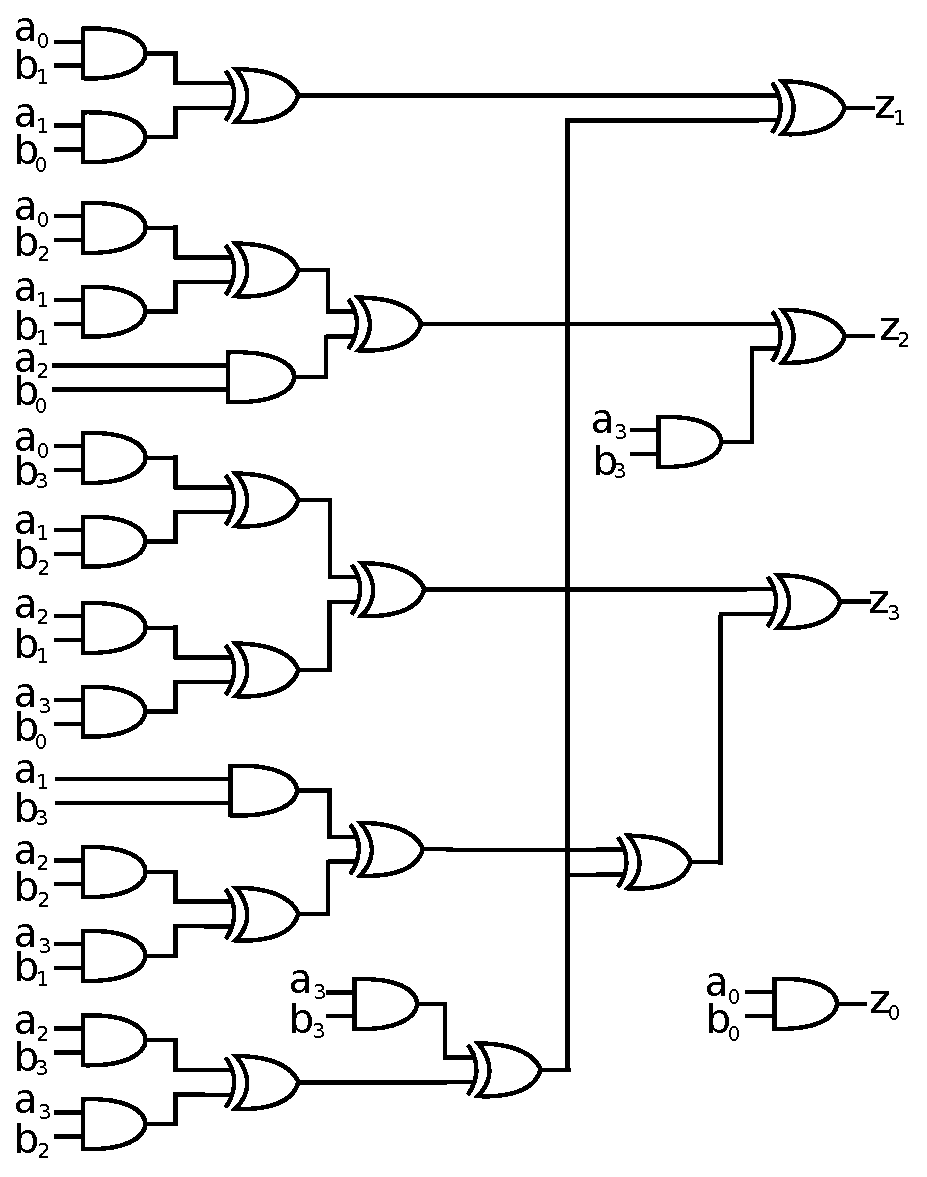
\includegraphics[scale=0.50]{figures/mul4bit.eps}
	\end{center}
	\caption{Mastrovito multiplier over $\mathbb{F}_{2^4}$.}
	\label{fig:mas4}
\end{figure}

Its corresponding composite field design with decomposition $\mathbb{F}_{(2^2)^{2}}$ is shown in Figure \ref{fig:mas22}.
Each block in Fig.\ref{fig:mas22} represents a $2$-bit operation internally, where 
$\times$ represents an $m$-bit multiplier and $+$ represents an $m$-bit adder. 

\begin{sidewaysfigure}
%\begin{figure}[h]
\centerline{
\includegraphics[scale=0.50]{./figures/cfmultiplier.eps}
}
\caption{Mastrovito multiplier over $\mathbb{F}_{(2^2)^2}$}
\label{fig:mas22}
%\end{figure}
\end{sidewaysfigure} 

%%%%%%%%%%%%%%%%%%%%%%%%%%%%%%%%%%%%%%%%%%%%%%
%%%%%%%%%%%%%%%%%%%%%%%%%%%%%%%%%%%%%%%%%%%%%%
%%%%%%%%%%%%%%%%%%%%%%%%%%%%%%%%%%%%%%%%%%%%%%
\section{Problem Formulation and Hierarchy Verification}
\label{sec:setup}

Let us again take the multiplier verification problem as example. 
The {\it specification} $S = A \cdot B \pmod{ P(x)}$ is already given in polynomial form (word level).
The {\it implementation} is available at two different abstraction 
levels: one at the bit-level (ground field $\mathbb{F}_{2^m}$ adders and
multipliers) and one at the higher-level at $\mathbb{F}_{(2^m)^n}$. 
Using this information, we derive constraints (polynomials) $Z$ corresponding to the circuit. 
Our verification problem is to prove/disprove that for all values of the inputs 
$A =\{a_0, \dots a_{k-1}\}, ~B=\{b_0, \dots b_{k-1}\}$, 
the circuit implementation $Z$ correctly computes the multiplication $S$.

As we can notice from Figure \ref{fig:mas22}, the entire composite field circuit is constructed
on lower level building-blocks (adders and multipliers).
Therefore, we have two verification objectives: low level circuits and
higher-level interconnection of the lower-level blocks.

{\bf Verification of low level circuits over $\mathbb{F}_{2^m}$:}

Low level building-blocks consist of adders and multipliers over $\mathbb{F}_{2^m}$.
These circuits are implemented at gate-level and are nothing special 
as the regular finite field circuits we verified before. 
Therefore, we can simply employ the same methods described in Chapter \ref{ch:date}
to formulate the verification test as membership testing of 
the property polynomial ($S+Z=0$). 
When the correctness of low level circuits is certified, we can conduct the
high level verification over $\mathbb{F}_{(2^m)^n}$.

{\bf Verification of higher-level interconnection over $\mathbb{F}_{(2^m)^n}$:}
The difficulty of verifying the composite field circuits 
lies in the verification of high level interconnection of low level building-blocks.
Specifically, due to the presence of hierarchy of composite field circuits, 
the constraints derived from the high level interconnection contain
both gate-level and word-level abstractions. For example, in Figure \ref{fig:mas22},
the circuit hierarchy can be described as follows:
\begin{eqnarray}\label{eqn:compf}
	a_{00}=a_0+a_3 \nonumber  \\
	a_{01}=a_2+a_3 \nonumber  \\
	a_{10}=a_1+a_3  \nonumber  \\
	a_{11}=a_2 \nonumber  \\
	A_0=a_{00}+a_{01} \cdot \alpha ^5 	\nonumber  \\
	A_1=a_{10}+a_{11} \cdot \alpha ^5   \nonumber  \\
	b_{00}=b_0+b_3		\nonumber  \\
	b_{01}=b_2+b_3		\nonumber  \\
	b_{10}=b_1+b_3		\nonumber  \\
	b_{11}=b_2			\nonumber  \\
	B_0=b_{00}+b_{01} \cdot \alpha ^5		\nonumber  \\	 
	B_1=b_{10}+b_{11} \cdot \alpha ^5		\nonumber  \\
	C_0 = A_0\cdot B_1		\nonumber  \\
	C_1 = A_1\cdot B_0		\nonumber  \\
	C_2 = A_0\cdot B_0		\nonumber  \\
	C_3 = A_1\cdot B_1		\nonumber  \\
	C_4 = C_0 + C_1			\nonumber  \\
	C_5 = C_3 \cdot \alpha ^5	\nonumber  \\
	C_6 = C_3 \cdot \alpha ^5	\nonumber  \\
	Z_0 = C_{4}+C_{5}			\nonumber  \\
	Z_{1}=C_{2}+C_{6}			\nonumber  \\ 
\end{eqnarray}
where $a_0, \dots, a_3, b_0,\dots,b_3$ are variables in $\mathbb{F}_{2}$ (bits) while 
$A_0,A_1,B_0,B_1, C_{1},\dots, C_{6}$, $Z_{0}$, $Z_{1}$ are variables in $\mathbb{F}_{2^2}$ (words).
Therefore bit-level variables and word-level variables co-exist in the design.
As far as we know, there are no techniques that can verify design with different levels of abstraction.
This is mainly because BDD/SAT/AIG based approaches can only handle bit-level problems. 
SMT solvers, on the other hand, have no advantages to solve problems at bit-level. 
Besides, SMT solvers formulate every problem over rings instead of finite fields. 
Take Eqnations \ref{eqn:compf} for example, $C_0 = A_0\cdot B_1$ represents a $2$-bit finite field multiplication.
In SMT,  $C_0 = A_0\cdot B_1$ represents a $2$-bit integer multiplication. As we know, the multiplication over rings and over finite fields differs significantly.
 
Fortunately, due to the fact that both bits and words information can be formulated as polynomials,
this verification problem is algebraic in nature and therefore 
can be easily formulated as a system of polynomials and solved by ideal membership testing,
which is described in Algorithm \ref{alg:overall}.

\begin{Example}
		
	Our high-level verification problem is illustrated in Table \ref{tab:masvercf}. 
	Let $F$ denote all the polynomials representing {\it implementation}, {\it specification} and {\it vanishing polynomials}.
	Let $F_0$ denote the vanishing polynomials for primary inputs.
	After all the polynomials in $\{F\}$ are available, 
	we just need to check whether $S+Z$ is a member of the ideal $\langle F,F_0\rangle$.
	
	\begin{table}[t]
	\begin{center}
	\caption{Verification Setup over $\mathbb{F}_{(2^2)^2}$}\label{tab:masvercf}
	\begin{tabular}{|c | c|c|}
	\hline
	{\it implementation} & {\it specification} 	&  {\it vanishing polynomials}\\
	\hline
	$a_{00}+a_0+a_3$ & $A+a_0+a_1\cdot \alpha+a_2\cdot \alpha^2+a_3\cdot \alpha^3$   &$a_0^{2}-a_0$		\\
	$a_{01}+a_2+a_3$ & $B+b_0+b_1\cdot \alpha+b_2\cdot \alpha^2+b_3\cdot \alpha^3$ 	&$a_1^{2}-a_1$			\\
	$a_{10}+a_1+a_3$ &  $S+A\times B$ &$a_2^{2}-a_2$	\\
	$a_{11}+a_2$ &  &$a_3^{2}-a_3$	\\ 
	$A_0+a_{00}+a_{01} \cdot x^5$ & 	&$b_0^{2}-b_0$	\\ 
	$A_1+a_{10}+a_{11} \cdot x^5$ & 	&$b_1^{2}-b_1$\\
	$b_{00}+b_0+b_3$ & &$b_2^{2}-b_2$\\
	$b_{01}+b_2+b_3$ & &$b_3^{2}-b_3$\\
	$b_{10}+b_1+b_3$ & &\\
	$b_{11}+b_2$ & &\\
	$B_0+b_{00}+b_{01} \cdot x^5$ & &\\ 
	$B_1+b_{10}+b_{11} \cdot x^5$ & &\\
	$C_0 + A_0\cdot B_0$    &    &\\
	$C_1 + A_1\cdot B_0$		  &    \\
	$s_2 + A_1\cdot B_1$    &  &\\
	$C_3 + A_1\cdot B_1$		&  &\\
	$C_4 + C_0 + C_1$			& & \\
	$C_5 + C_3 \cdot \alpha ^5$	&  &\\
	$C_6 + C_3 \cdot \alpha ^5$	&  &\\
	$Z_0 + C_{4}+C_{5}$			& & \\
	$Z_{1}+C_{2}+C_{6}$			&  &\\ 
	$Z+Z_{0}+Z_{1}\cdot \alpha $ & &\\ 
	\hline
	\multicolumn{3}{|c|}{Property: $\mathbf{Z+S}$} \\
	\hline
	\end{tabular}
	\end{center}
	\end{table}

\end{Example}

\section{Experimental Results}\label{sec:experiment}

With the approach presented above, we have conducted experiments to
hierarchically verify Mastrovito multiplier implementations $M$
against the specification $S = A\cdot B \pmod{ P(x)}$. Our
verification setup is shown of Table \ref{tab:masvercf}. The implementation
is given as a circuit over $\mathbb{F}_{(2^m)^n}$. With the given hierarchy
information, we construct the polynomials representing high level
designs $M_H$ over $\mathbb{F}_{(2^m)^n}$ and low level designs $M_L$
over $\mathbb{F}_{2^m}$ separately. 

For high level designs $M_H$, the specification polynomials $S = A \cdot B \pmod{ P(x)}$ is used.
In contrast, for low level designs $M_L$ over $\mathbb{F}_{2^m}$, the specification
polynomials $S_L  = A_{m} \cdot B_{m} \pmod{ Q(x)}$ is used, of which,
$A_{m},B_{m}$ represents the $m$-bit inputs for low level building-block circuits;
$Q(x)$ is the primitive polynomial of $\mathbb{F}_{2^m}$.
Then vanishing polynomials ${a_0^2-a_0,\dots,a_{k-1}^2-a_{k-1}, b_0^2-b_0,b_{k-1}^2-b_{k-1}}$ 
are then appended to $M_H$ and $M_L$ at different levels of design.
We use {\sc singular} \cite{DGPS} to conduct polynomial reduction. 
When the circuits are correctly designed, we do observe that reduction result is $0$, 
proving the equivalence. 

Our experiments are conducted on a desktop with $2.40$GHz CPU and $8$GB
memory running $64$-bit Linux. The time-out limit is set as $24$ hours. 

The verification of low level circuits is the same as the one shown in Table \ref{tab:ourmas}. 
The number of low level design units is shown in Table \ref{tbl:stats}. Note
that this number is determined by $n$, which means $\mathbb{F}_{(2^{m_1})^n}$
and $\mathbb{F}_{(2^{m_2})^n}$ have the same number of low level design units,
even if $m_1 \neq m_2$.

Since high level verification cannot be solved by any other technique, we only show the results of our approach.
Table \ref{tbl:modvsword} shows the runtime of high level designs verification over $\mathbb{F}_{(2^m)^n}$ 
for varying word-size $k=m\cdot n$. As shown in Table \ref{tbl:modvsword}, with our approach, 
we are able to prove the correctness of finite field circuits for up to $1024$-bit 
with decomposition $\mathbb{F}_{(2^{32})^{32}}$.

\begin{sidewaystable} 
%\begin{table}[h!]
\begin{center}
\caption{Verification of Mastrovito multiplier over $\mathbb{F}_{(2^m)^n}$ Using Proposed Approach. All times are given in seconds.}
\label{tbl:modvsword}
\begin{tabular}{||c|c|c||c|c|c||c|c|c||c|c|c||c|c|c||c|c|c||} 
\hline
\multicolumn{3}{||c||}{32}&\multicolumn{3}{c||}{64} &
\multicolumn{3}{c||}{128}&\multicolumn{3}{c||}{256} &
\multicolumn{3}{c||}{512}&\multicolumn{3}{c||}{1024}     \\
\hline
$m$& $n$ & time& $m$& $n$ & time& $m$& $n$ & time& $m$& $n$ & time& $m$& $n$ & time& $m$& $n$ & time \\
\hline
$2$  & $16$ & $7.55$ & $2$ & $32$ &$879.83$& $2$& $64$ & $\ast$& $2$ & $128$ & $\ast$ & $2$&$256$&$\ast$ & $2$&$512$&$\ast$\\
\hline
$4$  & $8$  & $0.12$ & $4$ & $16$ & $10.81$& $4$& $32$&$1619.51$& $4$ & $64$  & $\ast$ & $4$&$128$&$\ast$ & $4$&$256$&$\ast$\\
\hline
$8$  & $4$  & $0.01$ & $8$ & $8$  & $0.46$ & $8$& $16$ &$35.04$& $8$ & $32$  & $2664.56$ & $8$&$64$ &$\ast$ & $8$&$128$&$\ast$\\
\hline
$16$ & $2$  & $0.01$ & $16$& $4$  & $0.15$ &$16$& $8$  & $3.25$&$16$ & $16$  &$147.84$&$16$&$32$ &$11510$ & $16$&$64$&$\ast$\\
\hline
 -   & -    & -      & $32$& $2$  & $0.11$ &$32$& $4$  & $2.14$&$32$ & $8$   & $37.71$&$32$&$16$ &$1166.10$&$32$ &$32$ & $75336$  \\
\hline
\end{tabular}
\end{center}

\begin{center}
\caption{Statistics of Designs over $\mathbb{F}_{2^m}$}
\label{tbl:stats}
\begin{tabular}{|c|c|c|c|c|c|c|c|} 
\hline
$n$ & 2 & 4 & 8 & 16 & 32 \\
\hline
\#Multipliers  & $6$ & $36$ & $168$ & $720$ & $2976$ \\
\hline
\#Adders       & $3$ & $27$ & $147$ & $675$ & $2883$  \\
\hline
\end{tabular}
\end{center}
\end{sidewaystable}

\section{Conclusions}
This chapter has targeted the implementation verification of
hierarchically designed composite finite field circuits. 
Decomposing the finite field $\mathbb{F}_{2^k}$ as $\mathbb{F}_{(2^m)^n}$ 
introduces a hierarchical abstraction. Our approach requires that
this hierarchy information be made available. Then, we formulate the
verification problem using the polynomial reduction
as a ideal membership testing at different levels of abstraction.
First we verify low-level adders and
multipliers at $\mathbb{F}_{2^m}$, and then verify the high-level
interconnections between these blocks at $\mathbb{F}_{(2^m)^n}$. Using our
approach, we can verify the correctness of up to 1024-bit multipliers
where other contemporary techniques are not capable of verifying such circuits.
This work was presented in \cite{lv:hldvt2011}.
